%++++++++++++++++++++++++++++++++++++++++
% Don't modify this section unless you know what you're doing!
\documentclass[letterpaper,12pt]{article}
\usepackage{tabularx} % extra features for tabular environment
\usepackage{amsmath}  % improve math presentation
\usepackage{graphicx} % takes care of graphic including machinery
\usepackage[margin=1in,letterpaper]{geometry} % decreases margins
\usepackage{cite} % takes care of citations
\usepackage[final]{hyperref} % adds hyper links inside the generated pdf file



\hypersetup{
	colorlinks=true,       % false: boxed links; true: colored links
	linkcolor=blue,        % color of internal links
	citecolor=blue,        % color of links to bibliography
	filecolor=magenta,     % color of file links
	urlcolor=blue         
}
%++++++++++++++++++++++++++++++++++++++++


%Blackboard Letters

\newcommand{\R}{\ensuremath{\mathbb{R}}}
\newcommand{\C}{\ensuremath{\mathbb{C}}}
\newcommand{\Z}{\ensuremath{\mathbb{Z}}}
\newcommand{\Q}{\mathbb{Q}}
\newcommand{\N}{\mathbb{N}}
\newcommand{\F}{\mathbb{F}}
\newcommand{\W}{\mathbb{W}}


% Theorem / Lemmas et cetera

\newtheorem{thm}{Theorem}[section]
\newtheorem{conj}[thm]{Conjecture}
\newtheorem{cor}[thm]{Corollary}
\newtheorem{lem}[thm]{Lemma}
\newtheorem{prop}[thm]{Proposition}
\newtheorem{exa}[thm]{Example}
\newtheorem{defi}[thm]{Definition}
\newtheorem{exe}[thm]{Exercise}
\newtheorem{rek}[thm]{Remark}
\newtheorem{que}[thm]{Question}
\newtheorem{prob}[thm]{Problem}
\newtheorem{cla}[thm]{Claim}


\begin{document}

\title{C1 Assignment 2 Report}
\author{1104630}
\date{\today}
\maketitle


\section{Theory}

\subsection{DIRK Methods and Order of Convergence}

In this assignment, we were interested in the experimental order of convergence and the error of approximated solutions to the initial value problem,
\[
y'(t) = f(t, y(t)), \quad	 t_0 = t(0).
\]
where we investigated two different functions $f$.
\begin{align}
f(t, u) &= 1 - \cos(t)(\cos(t) - 1) - u^2, \quad u_0 = 0, \: T= 2\pi \\ 
f(t, u) &= 1 - \cos(t)(\cos(t) - e^{\lambda t}) - e^{-2 \lambda t}u^2 + \lambda u, \quad u_0 = 0, \: T = 10, \: \lambda = -0.1
\end{align}

Both these equations can be solved analytically which allowed us to calculate the error between the approximated solution and the exact solution.

We considered the following five diagonally implicit Runge-Kutta methods:

\begin{description}
	\item[Forward Euler] \hfill \\
		An explicit method. Using the Taylor expansion, it can be shown that the theoretical order of convergence for this method is 1.
		
	\item[Backward Euler] \hfill \\
		An implicit method. Using the Taylor expansion, it can be shown that the theoretical order of convergence for this method is 1.
		
	\item[Crank-Nicholson] \hfill \\
		An implicit method. Also known as Gauss-Legendre method, this method arises from considering the integral trapezoidal quadrature rule. The theoretical order of convergence for this method is 2.
	
	\item[3-step Heun] \hfill \\
		An explicit method. The theoretical order of convergence for this method is 3. 
		
	\item[2-step DIRK] \hfill \\
		An implicit method. The theoretical order of convergence of this method is 2.
		
\end{description}


\section{Results}		

\subsection{Maximum Error vs. eoc}

The following results tables give the maximum error and the experimental order of convergence for each of the models and DIRK schemes for $\tau = 0.1 \times 2^{-12}$.

\begin{table}[ht]
\caption{Equation 1} % title of Table
\centering % used for centering table
\begin{tabular}{c c c} % centered columns
\hline\hline %inserts double horizontal lines
Scheme & Maximum Error & eoc \\ [0.5ex] % inserts table
%heading
\hline % inserts single horizontal line

      Forward Euler &      $1.20 \times 10^{-5}$ & 0.999956	\\
     Backward Euler &      $1.20 \times 10^{-5}$ & 0.999864 \\
  	Crank-Nicholson &      $5.60 \times 10^{-8}$ & 1.99265  \\
   	   3-stage Heun &     $2.70 \times 10^{-10}$ & -2.29754 \\
       2-stage DIRK &      $1.02 \times 10^{-7}$ & 1.996 \\


\hline %inserts single line
\end{tabular}
\label{table:nonlin} % is used to refer this table in the text
\end{table}


\begin{table}[ht]
\caption{Equation 2} % title of Table
\centering % used for centering table
\begin{tabular}{c c c} % centered columns
\hline\hline %inserts double horizontal lines
Scheme & Maximum Error & eoc \\ [0.5ex] % inserts table
%heading
\hline % inserts single horizontal line

      Forward Euler &      $1.60 \times 10^{-3}$ & 1.00479 \\
     Backward Euler &      $9.41 \times 10^{-4}$ & 1.00319 \\
  	Crank-Nicholson &      $1.27 \times 10^{-3}$ & 1.00385 \\
   	   3-stage Heun &      $1.51 \times 10^{-9}$ & -2.18845 \\
       2-stage DIRK &      $2.00 \times 10^{-3}$ & 1.00624 \\


\hline %inserts single line
\end{tabular}
\label{table:nonlin} % is used to refer this table in the text
\end{table}

From the tables we see that eoc of Forward Euler and Backward Euler converge. From the values in the terminal, we also see that the 3-stage Heun converges initially but eventually the numerical errors causes the eoc to not converge. 

However, there are some unexpected results for Crank-Nicholson and 2-stage DIRK as the eoc for the two models do not converge to the same value. It is probable that the implementation for implicit methods is wrong.


\section{Approximation Error over Time}

For each DIRK scheme, we graphed the $\log$-approximation error of the approximate solution to the IVP against the time.


\centerline{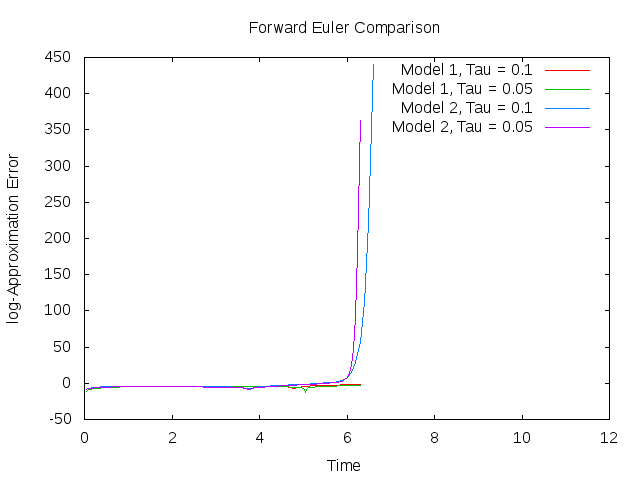
\includegraphics[scale = 0.5]{FE.png}}

\centerline{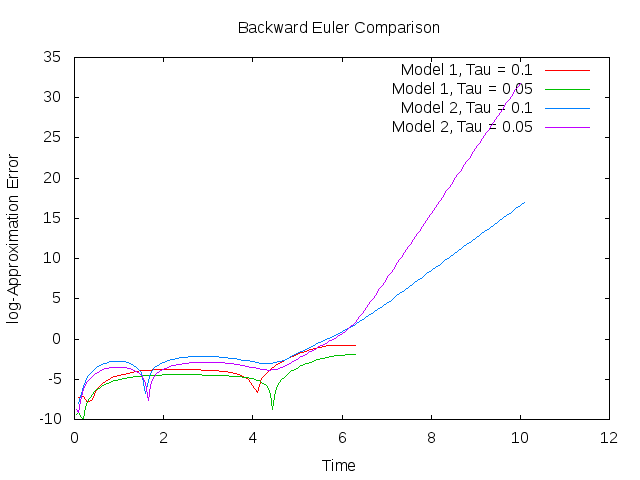
\includegraphics[scale = 0.5]{BE.png}}

\centerline{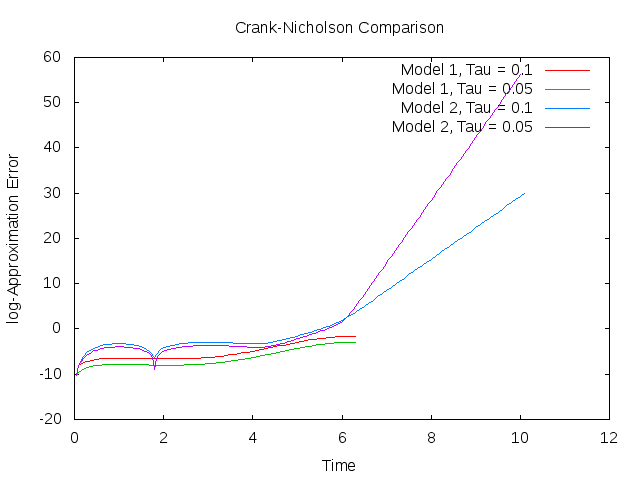
\includegraphics[scale = 0.5]{CN.png}}

\centerline{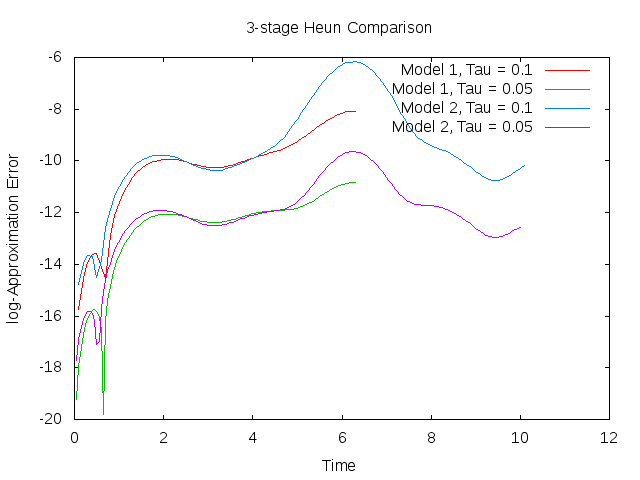
\includegraphics[scale = 0.5]{Heun3.png}}

\centerline{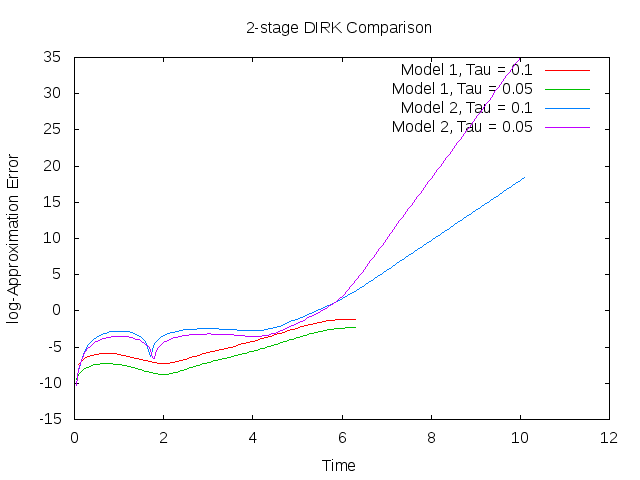
\includegraphics[scale = 0.5]{2DIRK.png}}

We originally thought that the graphs would be increasing as time increased as the approximation  and numerical errors should lead to increased error in the approximation of the solution. However, apart from the Forward Euler method, the graphs are quite erratic, with sharp decreases at certain time steps. This may be due to the fact that approximation error at a given time step could be cancelling out previous approximation errors. For example, as the exact solution for the second model is $e^{-\lambda t } \sin(t)$ which oscillates, so the changing sign of the derivative could cause the errors to cancel. 


\section{External Libraries}

Although \texttt{odeint} was installed, there was not enough time to compare the library with the implementation.


\end{document}
